\chapter{Resultados Preliminares}
\label{cap:resultados}

Reúnem-se neste capítulo os resultados já obtidos com o modelo descrito no
Capítulo~\ref{cap:modelagem}.

Os resultados aqui reunidos foram obtidos em duas corridas independentes, com
alimentações de razão molar \num{4}:\num{1} e \num{6}:\num{1}. A primeira
corresponde à condição em que \textcite{Melo2023} determinou a constante
cinética e é, por isso, a adotada no Capítulo~\ref{cap:modelagem}; a segunda foi
conduzida antes dessa constatação. A comparação entre as duas, apresentada na
Seção~\ref{sec:invariancia}, constitui um teste de verificação adicional, e os
valores reportados adiante são comuns a ambas.

A exposição segue a ordem em que os testes foram
conduzidos: primeiro a verificação do campo de velocidade, depois a dos
balanços de massa, e por fim a caracterização do regime de operação, que
constitui o resultado central do trabalho até o momento.

\section{Verificação hidrodinâmica}

O campo de velocidade foi verificado contra a solução analítica de Poiseuille
para canal plano,

\begin{equation}
u(y) = 6\,\bar{u}\,\frac{y}{H}\left(1 - \frac{y}{H}\right)
\label{eq:poiseuille}
\end{equation}

\noindent
por meio de um perfil transversal medido a \SI{49}{\milli\meter} da entrada,
apresentado na Figura~\ref{fig:poiseuille}.

\begin{figure}[htb]
\centering
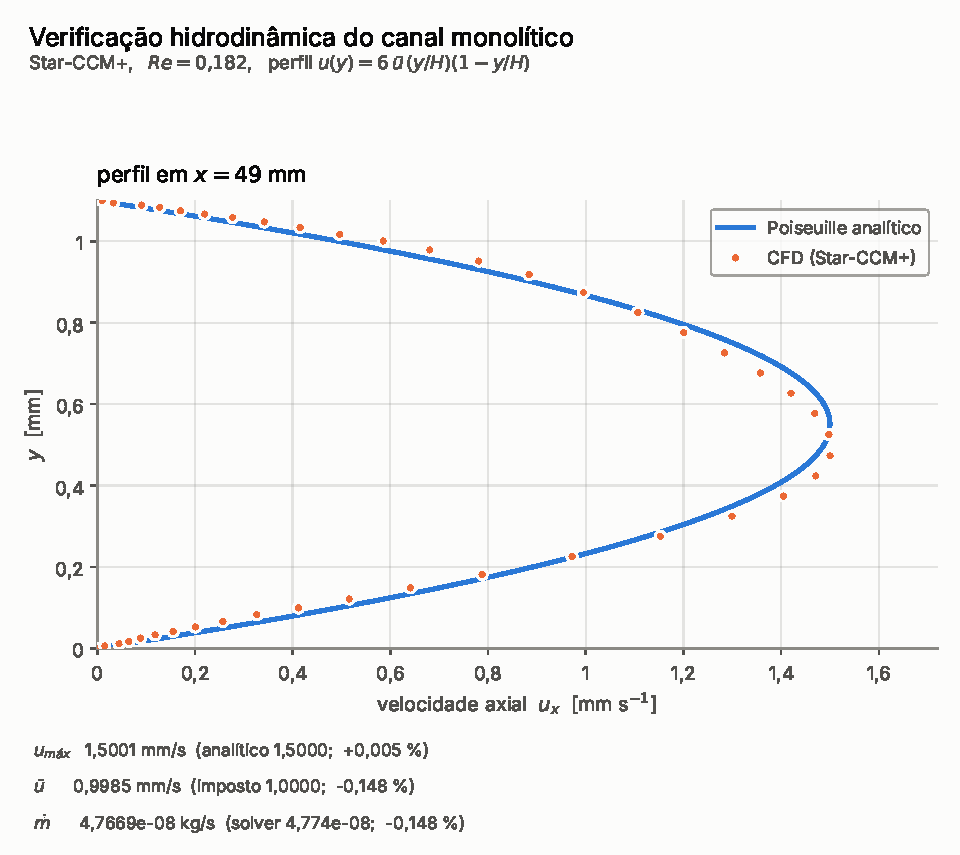
\includegraphics[width=0.74\textwidth]{fig6_poiseuille_fase3.pdf}
\caption{Perfil transversal de velocidade axial em $x = \SI{49}{\milli\meter}$,
comparado à solução analítica de Poiseuille para canal plano}
\label{fig:poiseuille}
\end{figure}

A concordância é satisfatória nas três grandezas integrais verificadas. A
velocidade máxima medida vale \SI{1.5001}{\milli\meter\per\second}, contra
$1{,}5\,\bar{u} = \SI{1.5000}{\milli\meter\per\second}$ previstos, diferença de
\SI{0.005}{\percent}. A integração do perfil fornece velocidade média de
\SI{0.9985}{\milli\meter\per\second}, \SI{0.15}{\percent} abaixo do valor
imposto na entrada, e vazão mássica de
\SI{4.767e-8}{\kilogram\per\second}, também \SI{0.15}{\percent} abaixo da
registrada pelo solver nas duas fronteiras.

Ponto a ponto, os valores junto às paredes apresentam dispersão maior, da ordem
de \SI{20}{\percent} nas primeiras células. O exame dessa dispersão mostra que
ela corresponde a um deslocamento aparente de aproximadamente
\SI{9}{\micro\meter} entre a coordenada reportada pela sonda de linha e a
posição física das células da malha, e não a um erro da solução: um ajuste
parabólico aos valores de célula fornece raízes em \SI{7.9}{\micro\meter} e
\SI{1109.5}{\micro\meter}, ou seja, altura de canal de
\SI{1101.6}{\micro\meter} contra os \SI{1100}{\micro\meter} nominais. Como as
três grandezas integrais concordam dentro de \SI{0.15}{\percent}, considera-se
o campo de velocidade verificado.

A perda de carga calculada foi de \SI{5.463}{\pascal}, contra
\SI{5.207}{\pascal} da solução de Hagen-Poiseuille,
$\Delta P = 12\,\mu\,\bar{u}\,L/H^2$, diferença de \SI{4.9}{\percent}. Essa
discrepância convive com a concordância de \SI{0.15}{\percent} nas grandezas
cinemáticas, e não compromete o transporte de espécies, que depende do campo de
velocidade e não da pressão.

Registre-se, por fim, uma observação de caráter prático a respeito da perda de
carga. Ela não constitui indicador de qualidade de malha neste problema: a
solução plenamente desenvolvida é um perfil parabólico, que um esquema de
volumes finitos de segunda ordem integra exatamente em qualquer discretização.
Obteve-se, de fato, valor idêntico até a sétima casa decimal em malhas com e sem
camadas prismáticas. O refino junto à parede, indispensável ao transporte de
espécies pelas razões da Seção~\ref{sec:verificacao}, é invisível a esse teste.

\section{Conservação de massa e independência de malha}

A consistência estequiométrica, definida pela Equação~\eqref{eq:esteq}, foi
monitorada ao longo de todas as simulações. Os valores medidos situaram-se entre
\num{1.00455} e \num{1.00462}, contra o valor teórico de \num{1.004587}, o que
representa concordância de \SI{0.009}{\percent}. A estabilidade dessa razão ao
longo de toda a marcha temporal, desde os primeiros décimos de segundo até o
regime permanente, constitui a evidência mais direta de que o transporte de
espécies conserva massa no modelo.

A independência de malha foi avaliada por meio da reprodução do resultado
central em duas configurações distintas, cujos parâmetros e resultados estão
reunidos na Tabela~\ref{tab:malhas}. As duas configurações diferem não apenas na
discretização, mas também na composição de alimentação, e ainda assim
concordam dentro de \SI{2}{\percent}.

\begin{table}[htb]
\centering
\caption{Independência de malha e de composição de alimentação}
\label{tab:malhas}
\begin{tabular}{l c c c c}
\toprule
Configuração & Primeira célula & Alimentação & $C_w/C_b$ & $Da$ \\
\midrule
Sem camadas prismáticas & \SI{50}{\micro\meter}  & \num{4}:\num{1} molar & \num{0.578} & \num{0.730} \\
Com camadas prismáticas & \SI{2.8}{\micro\meter} & \num{6}:\num{1} molar & \num{0.574} & \num{0.743} \\
\bottomrule
\end{tabular}
\end{table}

\subsection{Invariância com a composição de alimentação}
\label{sec:invariancia}

A Seção~\ref{sec:difusividades} argumenta que, por se tratar de cinética de
pseudo-primeira ordem, tanto o número de Damköhler quanto a conversão
fracionária são razões e independem, em primeira aproximação, do valor absoluto
da concentração de entrada. A disponibilidade de duas corridas convergidas com
alimentações distintas permite submeter esse argumento a teste.

A grandeza adequada para a comparação é o empobrecimento relativo do domínio em
regime permanente, $(Y_{in} - Y_{bulk})/Y_{in}$, que deve ser idêntico nas duas
corridas caso a invariância se verifique. A Tabela~\ref{tab:invariancia} reúne
os valores medidos.

\begin{table}[htb]
\centering
\caption{Empobrecimento relativo do domínio em regime permanente para duas
composições de alimentação}
\label{tab:invariancia}
\begin{tabular}{c c c c}
\toprule
Alimentação & $Y_{TG}$ na entrada & $Y_{TG}$ no domínio & Queda relativa \\
\midrule
\num{4}:\num{1} molar & \num{0.8719} & \num{0.848043} & \SI{2.7363}{\percent} \\
\num{6}:\num{1} molar & \num{0.8194} & \num{0.796979} & \SI{2.7363}{\percent} \\
\bottomrule
\end{tabular}
\end{table}

As duas corridas concordam em quatro casas decimais, com discrepância de
\SI{0.001}{\percent}. A invariância prevista pelo argumento cinético verifica-se,
portanto, de forma essencialmente exata, e os valores de $Da$ e de $X_{TG}$
reportados nas seções seguintes valem para ambas as composições.

Registre-se que a concordância é mais estreita do que a de qualquer outro teste
de verificação aplicado ao modelo, incluindo a independência de malha. Isso é
esperado: trata-se da mesma malha e do mesmo conjunto de equações, diferindo
apenas o valor numérico de uma condição de contorno sobre a qual a solução, por
construção, deveria ser linear.

O balanço global de massa, Equação~\eqref{eq:balanco}, foi verificado em regime
permanente. A marcha foi conduzida até \SI{303}{\second}, instante em que o
inventário do domínio deixa de evoluir:

\begin{equation}
\frac{\mathrm{d}M_{TG}}{\mathrm{d}t} = \SI{-2.21e-14}{\kilogram\per\second}
= \SI{0.004}{\percent} \text{ do fluxo de parede}
\end{equation}

Nessa condição a Equação~\eqref{eq:balanco} reduz-se à forma
$\dot{m}\,(Y_{\text{ent}} - Y_{\text{sai}}) = |\oint J\,\mathrm{d}A|$, e o
fechamento foi confirmado pela integração do perfil transversal apresentado na
Seção~\ref{sec:camadalimite}.

\section{Regime de operação}

O resultado central do trabalho decorre da leitura das concentrações de
triglicerídeo junto à parede catalítica e no seio do fluido, e da aplicação da
Equação~\eqref{eq:cwcb}. A Tabela~\ref{tab:daresultado} reúne os valores
medidos em regime permanente nas duas corridas.

\begin{table}[htb]
\centering
\caption{Concentrações em regime permanente e número de Damköhler resultante}
\label{tab:daresultado}
\begin{tabular}{l c c}
\toprule
 & \num{4}:\num{1} molar & \num{6}:\num{1} molar \\
\midrule
$Y_{TG}$ na entrada             & \num{0.8719}   & \num{0.8194}   \\
$Y_{TG}$ na parede              & \num{0.481093} & \num{0.452120} \\
$Y_{TG}$ no domínio             & \num{0.848043} & \num{0.796979} \\
\midrule
$C_w/C_b$                       & \num{0.567299} & \num{0.567292} \\
$Da$                            & \num{0.7627}   & \num{0.7628}   \\
$X_{TG}$                        & \SI{1.4016}{\percent} & \SI{1.4016}{\percent} \\
\bottomrule
\end{tabular}
\end{table}

As duas corridas concordam em cinco a seis algarismos significativos, o que
confirma a invariância discutida na Seção~\ref{sec:invariancia}. Adota-se
daqui em diante

\begin{equation}
\boxed{Da = 0{,}76}
\label{eq:daresultado}
\end{equation}

O sistema opera, portanto, em \textbf{regime misto}. A resistência cinética e a
resistência ao transporte externo são da mesma ordem de grandeza, e a
concentração de triglicerídeo junto à superfície catalítica é \SI{43}{\percent}
menor que a do seio do fluido. Existe um gradiente substancial a ser vencido, e
é esse gradiente que confere função à geometria monolítica.

Convém contrastar esse valor com o que se obtinha na etapa anterior do trabalho.
Utilizando-se os parâmetros cinéticos de \textcite{Allain2016}, determinados
para ZnAl$_2$O$_4$ e extrapolados para as condições do canal, o número de
Damköhler resultava em \num{0.003}, valor que situa o sistema sob controle
cinético estrito. Nesse regime não há gradiente apreciável de concentração entre
a parede e o seio do fluido, e a área adicional oferecida pelo monólito não se
converte em desempenho. A Tabela~\ref{tab:regimes} resume a comparação.

\begin{table}[htb]
\centering
\caption{Regime de operação em função da cinética adotada}
\label{tab:regimes}
\begin{tabular}{l l c l}
\toprule
Etapa & Catalisador & $Da$ & Regime \\
\midrule
Anterior & ZnAl$_2$O$_4$ \parencite{Allain2016}, extrapolado & \num{0.003} & controle cinético \\
Atual    & CaO \parencite{Melo2023}, medido no laboratório   & \num{0.76}  & misto \\
\bottomrule
\end{tabular}
\end{table}

Uma ressalva de leitura é necessária. O valor de $Da = \num{0.003}$ da primeira
linha não descreve o sistema de \textcite{Allain2016}, e sim o canal monolítico
aqui simulado operando com os parâmetros cinéticos daqueles autores
extrapolados para \SI{65}{\celsius}. No sistema que eles próprios estudaram,
um leito fixo de partículas em temperatura muito superior, a conclusão foi de
limitação conjunta por difusão e cinética. A discrepância, portanto, não é
entre este trabalho e a fonte, e sim entre duas configurações de reator
distintas alimentadas pela mesma cinética.

A diferença entre as duas linhas da Tabela~\ref{tab:regimes} é de mais de duas
ordens de grandeza, e dela depende a própria justificativa da configuração de
reator investigada. O emprego de parâmetros cinéticos obtidos com o catalisador
efetivamente utilizado no laboratório, em lugar de valores extrapolados da
literatura para um sólido distinto, mostrou-se decisivo para a conclusão.

\subsection{Corroboração experimental}

O regime identificado encontra apoio em evidência experimental independente.
Operando um reator monolítico de múltiplos canais com óxido de estrôncio,
\textcite{Firth2014} observou dependência forte da taxa de reação com a vazão
de alimentação e concluiu, a partir dela, que a reação permanecia limitada por
transferência de massa. A dependência da taxa com a vazão é precisamente a
assinatura do controle por transporte externo: alterar a vazão altera a
espessura da camada-limite de concentração, e portanto o coeficiente de
transferência de massa, sem afetar a cinética na superfície.

Trata-se de catalisador distinto e de temperatura muito superior à aqui
simulada, de modo que os valores não são comparáveis. O que se transfere é a
natureza do regime: em um reator monolítico de parede catalítica aplicado à
transesterificação, o transporte externo participa do controle da conversão. É
essa a mesma conclusão a que conduz o $Da = \num{0.76}$ medido neste trabalho,
obtida por caminho inteiramente diferente.

\section{Camada-limite de concentração}
\label{sec:camadalimite}

A Figura~\ref{fig:camadalimite} apresenta o perfil transversal de fração mássica
de triglicerídeo medido a \SI{49}{\milli\meter} da entrada, acompanhado do
perfil de velocidade na mesma seção e da contribuição local de cada posição à
média ponderada por vazão.

\begin{figure}[htb]
\centering
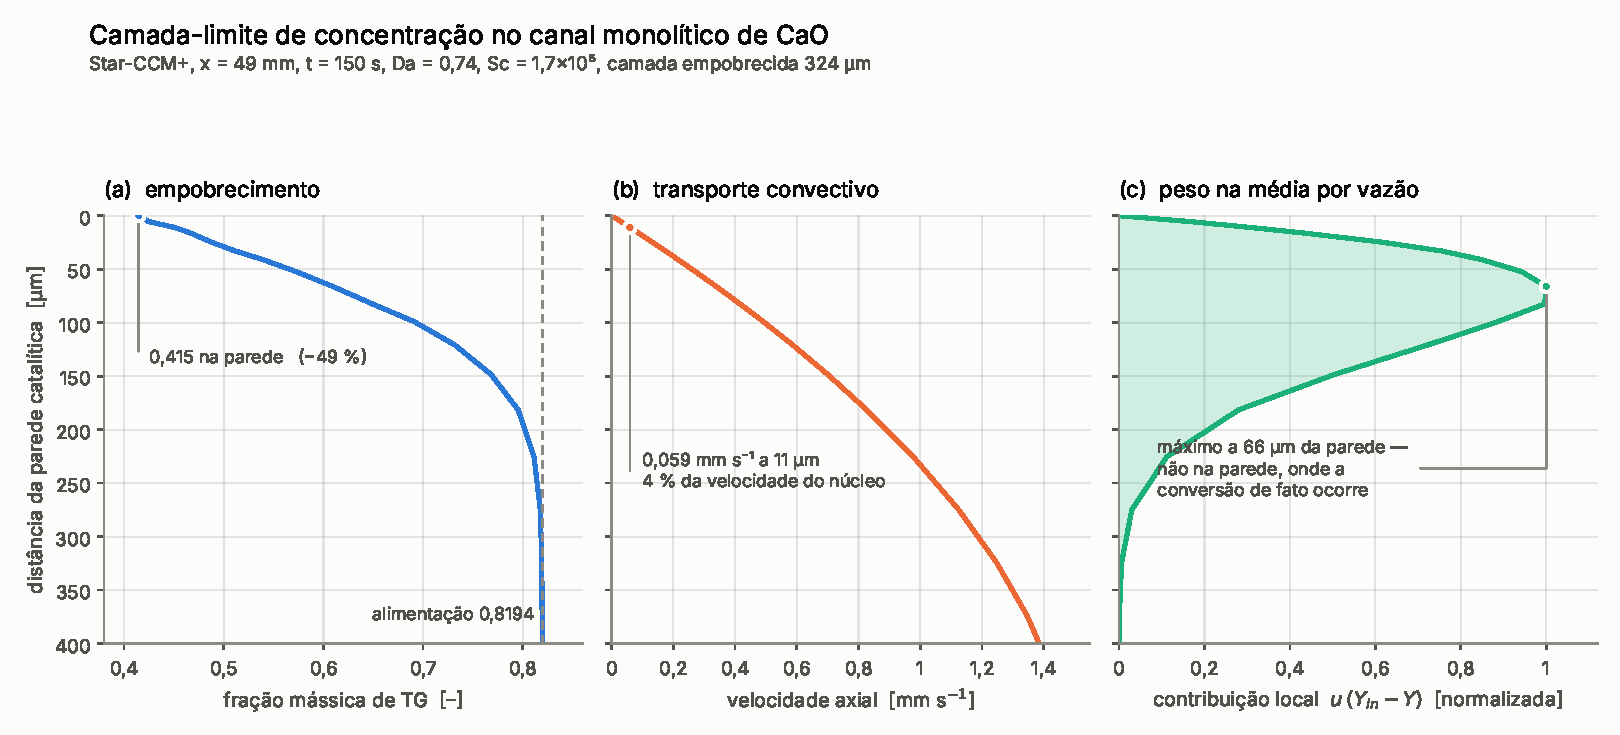
\includegraphics[width=\textwidth]{fig4_camada_limite_x49mm.pdf}
\caption{Camada-limite de concentração no canal monolítico de CaO, a
\SI{49}{\milli\meter} da entrada. (a)~fração mássica de triglicerídeo;
(b)~perfil de velocidade axial; (c)~contribuição local à média ponderada por
vazão}
\label{fig:camadalimite}
\end{figure}

A camada empobrecida tem espessura de \SI{324}{\micro\meter}, contra os
\SI{179}{\micro\meter} previstos pela solução de Lévêque,
Equação~\eqref{eq:leveque}, para regime permanente. A diferença tem origem
cinemática. Em \SI{150}{\second} de simulação, o regime permanente ainda não se
estabeleceu junto à parede, onde a velocidade local é muito pequena: o tempo de
trânsito do fluido situado a \SI{20}{\micro\meter} da superfície é de
\SI{458}{\second}, e a \SI{5}{\micro\meter}, de \SI{1833}{\second}. O tempo
característico do problema não é, portanto, o tempo de residência médio, igual a
$L/\bar{u} = \SI{50}{\second}$, mas o tempo de trânsito na região lenta, uma a
duas ordens de grandeza maior. Essa observação é relevante para o planejamento
de simulações futuras e para a interpretação de ensaios experimentais em
regime transiente.

O painel (c) da Figura~\ref{fig:camadalimite} merece comentário à parte. A
contribuição local à média ponderada por vazão, dada pelo produto
$u\,(Y_{\text{ent}} - Y)$, apresenta máximo a \SI{66}{\micro\meter} da parede, e
não sobre ela. A razão é simples e tem consequências que serão exploradas na
Seção~\ref{sec:reports}: o fluido mais empobrecido é justamente o mais lento, de
modo que a região onde a conversão de fato ocorre é a que menos pesa em qualquer
média ponderada pela vazão.

\section{Conversão por passe e limitação geométrica}

A conversão de triglicerídeo foi obtida diretamente da integral do fluxo de
parede,

\begin{equation}
X_{TG} = \frac{\left| \oint_{A_p} J_{TG}\, \mathrm{d}A \right|}{\dot{m}\, Y_{TG,\text{ent}}}
= \SI{1.40}{\percent}
\label{eq:conversao}
\end{equation}

\noindent
valor próximo de \SI{1.5}{\percent}, estimado analiticamente antes da simulação
pela combinação da solução de Lévêque com a cinética de parede.

O valor baixo não constitui deficiência do catalisador, e sim consequência
direta da relação entre o comprimento do canal e o comprimento de entrada
mássica. Com os parâmetros da Tabela~\ref{tab:propriedades},

\begin{align}
Re &= \frac{\rho\,\bar{u}\,D_h}{\mu} = 0{,}182 \nonumber\\
Sc &= \frac{\mu}{\rho\,D} = \num{1.73e5} \nonumber\\
Pe &= Re \cdot Sc = \num{3.1e4} \nonumber
\end{align}

\noindent
de modo que a Equação~\eqref{eq:entrada} fornece

\begin{equation}
L_e \approx 0{,}05 \times \SI{2.2e-3}{\meter} \times \num{3.1e4} = \SI{3.46}{\meter}
\end{equation}

\noindent
contra os \SI{50}{\milli\meter} do canal simulado, razão de \num{69}. A
camada-limite de concentração jamais chega a preencher a seção, e o núcleo do
escoamento deixa o canal praticamente na composição de alimentação.

Trata-se, a rigor, do resultado de projeto mais consequente obtido até aqui. O
número de Schmidt elevado, característico de óleos vegetais, implica que um
canal curto opera permanentemente na região de entrada mássica. Elevar a
conversão por passe exige atuar sobre $Pe$ ou sobre $L$, seja por meio de canais
mais longos, de velocidade superficial menor ou de reciclo. Aumentar
isoladamente a carga de catalisador tem retorno decrescente, uma vez que, já em
$Da = \num{0.76}$, o transporte externo responde por \SI{43}{\percent} da queda
de concentração disponível.

\section{Considerações metodológicas sobre a leitura de grandezas de fronteira}
\label{sec:reports}

O fechamento do balanço de massa descrito na Equação~\eqref{eq:balanco} exigiu
esforço desproporcional à sua aparente simplicidade, e as dificuldades
encontradas têm interesse que ultrapassa o presente trabalho. Registram-se aqui
por constituírem modos de falha que não se manifestam em nenhum dos indicadores
usuais de convergência.

Ao longo das simulações, três relatórios distintos de fração mássica de espécie,
todos avaliados em face de fronteira ou em objeto derivado, forneceram valores
incorretos, retornando aproximadamente a composição de alimentação. Em
contrapartida, as grandezas avaliadas sobre células permaneceram corretas e
mutuamente consistentes. A Tabela~\ref{tab:reports} sintetiza o comportamento
observado.

\begin{table}[htb]
\centering
\caption{Confiabilidade das grandezas de fração mássica avaliadas}
\label{tab:reports}
\begin{tabular}{l l l}
\toprule
Grandeza & Base de avaliação & Comportamento \\
\midrule
Média volumétrica de $Y_i$              & célula (região)        & correta \\
Integral de superfície de $J_i$         & função de campo        & correta \\
Média de superfície de $Y_i$ na parede  & face de fronteira      & retornou $Y_{\text{ent}}$ \\
Média ponderada por vazão na saída      & face de fronteira      & erro de fator \num{19} \\
Sonda de linha de $Y_i$                 & objeto derivado        & retornou $Y_{\text{ent}}$ \\
\bottomrule
\end{tabular}
\end{table}

O caso da média ponderada por vazão na saída possui, além da falha numérica, uma
fragilidade de natureza física já antecipada na Seção~\ref{sec:camadalimite}: o
fluido mais empobrecido é o mais lento, de modo que a região portadora da
informação de conversão quase não pesa na média, e o resultado fica à mercê de
qualquer contaminação pela composição especificada na fronteira.

Uma distinção útil emergiu da última corrida. O monitor de média de superfície
sobre a parede, isto é, a série temporal registrada a cada passo, permaneceu
cravado no valor da alimentação do primeiro ao último instante, ao passo que o
relatório instantâneo da mesma grandeza, consultado ao fim da corrida, forneceu
o valor correto de \num{0.481093}, confirmado pela integral do fluxo em seis
algarismos. Monitor e relatório podem, portanto, divergir, e a verificação
cruzada da Equação~\eqref{eq:cruzada} deve ser aplicada a ambos.

O caso da média de superfície sobre a parede é inequívoco. Ao retomar-se a
marcha a partir de um arquivo salvo, o relatório passou a retornar o valor exato
da composição de alimentação, \num{0.819400}, permanecendo congelado por três
mil passos de tempo, ao passo que a integral do fluxo sobre a mesma parede
seguia correta e fornecia, pela cadeia de funções de campo,
$Y_{TG}|_{\text{parede}} = \num{0.4521}$. Uma sonda de linha criada após a
retomada apresentou o mesmo defeito.

A prática que se consolidou ao longo do trabalho, e que se recomenda a quem
venha a montar modelos semelhantes, é a seguinte. Para fração mássica de
espécie, empregam-se exclusivamente grandezas avaliadas sobre células, a saber,
médias e integrais volumétricas sobre a região, e integrais de superfície de
funções de campo construídas sobre o próprio campo. A verificação cruzada que
detecta os três casos é barata e deve ser executada de rotina:

\begin{equation}
\text{média volumétrica de } Y_i \;\;\stackrel{!}{=}\;\; \frac{M_i}{\rho\, V}
\label{eq:cruzada}
\end{equation}

\noindent
com concordância esperada de cinco a seis algarismos significativos. Não havendo
concordância, o erro está no relatório, e não no modelo.
